%%%%%%%%%%%%%%%%%%%%%%%%%%%%%%%%%%%%%%%%%
% Short Sectioned Assignment
% LaTeX Template
% Version 1.0 (5/5/12)
%
% This template has been downloaded from:
% http://www.LaTeXTemplates.com
%
% Original author:
% Frits Wenneker (http://www.howtotex.com)
%
% License:
% CC BY-NC-SA 3.0 (http://creativecommons.org/licenses/by-nc-sa/3.0/)
%
%%%%%%%%%%%%%%%%%%%%%%%%%%%%%%%%%%%%%%%%%

%----------------------------------------------------------------------------------------
% PACKAGES AND OTHER DOCUMENT CONFIGURATIONS
%----------------------------------------------------------------------------------------

\documentclass[paper=a4, fontsize=11pt]{scrartcl} % A4 paper and 11pt font size

\usepackage[T1]{fontenc} % Use 8-bit encoding that has 256 glyphs
\usepackage{fourier} % Use the Adobe Utopia font for the document - comment this line to return to the LaTeX default
\usepackage[english]{babel} % English language/hyphenation
\usepackage{amsmath,amsfonts,amsthm} % Math packages
\usepackage[margin=0.7in]{geometry}

\usepackage{sectsty} % Allows customizing section commands
%\allsectionsfont{\centering \normalfont\scshape} % Make all sections centered, the default font and small caps

\usepackage{pgfplots}
\usepackage{tikz} % Работа с графикой
\usepackage{pgfplotstable}
\pgfplotsset{compat=1.3}

\usepackage{hyperref} %hyperlinks
\usepackage{float}
\usepackage{csquotes}
\usepackage{rotating}

\usepackage{color}
\usepackage{amsmath}
\usepackage{booktabs}
\usepackage[framemethod=TikZ]{mdframed}


\usepackage{array}
\newcolumntype{L}[1]{>{\raggedright\let\newline\\\arraybackslash\hspace*{0pt}}m{#1}}
\newcolumntype{C}[1]{>{\centering\let\newline\\\arraybackslash\hspace*{0pt}}m{#1}}
\newcolumntype{R}[1]{>{\raggedleft\let\newline\\\arraybackslash\hspace*{0pt}}m{#1}}

\usepackage{fancyhdr} % Custom headers and footers
\pagestyle{fancyplain} % Makes all pages in the document conform to the custom headers and footers
\fancyhead{} % No page header - if you want one, create it in the same way as the footers below
\fancyfoot[L]{Belino Xhafa, Christopher Chen, Josh Felizardo, \& Wenzhe (Harry) Xue} % Empty left footer
\fancyfoot[C]{} % Empty center footer
\fancyfoot[R]{\thepage} % Page numbering for right footer
\renewcommand{\headrulewidth}{0pt} % Remove header underlines
\renewcommand{\footrulewidth}{0pt} % Remove footer underlines
\setlength{\headheight}{10.6pt} % Customize the height of the header

\numberwithin{equation}{section} % Number equations within sections (i.e. 1.1, 1.2, 2.1, 2.2 instead of 1, 2, 3, 4)
\numberwithin{figure}{section} % Number figures within sections (i.e. 1.1, 1.2, 2.1, 2.2 instead of 1, 2, 3, 4)
\numberwithin{table}{section} % Number tables within sections (i.e. 1.1, 1.2, 2.1, 2.2 instead of 1, 2, 3, 4)

\setlength\parindent{0pt} % Removes all indentation from paragraphs - comment this line for an assignment with lots of text

\usepackage{graphicx}


%----------------------------------------------------------------------------------------
% TITLE SECTION
%----------------------------------------------------------------------------------------

\newcommand{\horrule}[1]{\rule{\linewidth}{#1}} % Create horizontal rule command with 1 argument of height
\newcommand{\prp}{\mathbb{P}}

\title{ 
\normalfont \normalsize 
\textsc{Harvard University, Stat 139, Spring 2016} \\ [25pt] % Your university, school and/or department name(s)
\horrule{0.5pt} \\[0.4cm] % Thin top horizontal rule
\huge Final Project: Analysis of Kobe Bryant's Shooting Performance \\ % The assignment title
\horrule{2pt} \\[0.5cm] % Thick bottom horizontal rule
}


\newenvironment{problem}[1]{\par\bigskip\noindent\textbf{Problem git 
#1.}\enskip\ignorespaces}{}

\mdfdefinestyle{MyFrame}{%
    linecolor=black,
    outerlinewidth=0.5pt,
    roundcorner=5pt,
    innertopmargin=\baselineskip,
    innerbottommargin=\baselineskip,
    innerrightmargin=15pt,
    innerleftmargin=15pt,
    backgroundcolor=gray!2!white}

\author{Belino Xhafa, Christopher Chen, Josh Felizardo, \& Wenzhe (Harry) Xue}
\date{\normalsize May 4, 2016} % Today's date or a custom date

\begin{document}

\maketitle % Print the title
\section{Research Questions}
\begin{itemize}
	\item What factors influenced whether Kobe Bryant made a given shot? Is Kobe especially talented at a particular type of shot?
	\item Kobe Bryant is a renowned ``clutch'' player. Is there a statistically significant difference between Kobe Bryant's accuracy when there are less than two minutes remaining in a given game compared to his overall accuracy? What about the fourth quarter and overtime?
	\item Is there a statistically significant relationship between Kobe's game performance and the ultimate result of a given game (on average)?
	\item Did his major injuries have a significant impact on his performance in the short/long term?
	\item Did Kobe's performance change depending on whether he was playing at home or away?
\end{itemize}
\section{Motivation}
\hspace*{1cm}Often considered one of the best players in NBA history, Kobe Bryant has become synonymous with many aspects of the game of basketball. While known as a prolific volume scorer, Kobe has also built a reputation as a clutch player, dictating his team's performance in the closing parts of each game. At the same time, there are many potential factors that could affect his performance in games, such as where he was playing, whether the Lakers won or lost, or whether he was suffering from injuries. In particular, Kobe has also been renowned as a remarkably tough player, so the effects of injuries on his performance would be especially interesting to consider. And given his recent retirement, we believe that researching the factors influencing (and influenced by) Kobe's shooting accuracy will prove to be a useful, relevant, and intriguing application of the statistical techniques learned in this class. 
\section{Hypotheses}
\section{Methods}
	\subsection{Dataset Used}
	\hspace*{1cm}The dataset used as the basis for our analysis was downloaded from the Kobe Bryant Shot Selection Kaggle competition \cite{kagglecompetition}.
	\subsection{Overview}
	Our code is divided into the following files as follows:
		\begin{itemize}
			\item \textbf{analysis.R} contains preliminary exploratory analysis of the datasets
			\item \textbf{cleaning.R} contains the commands we ran to clean/preprocess the data
			\item \textbf{hypothesis\_testing.R} contains various hypothesis tests for statistical significance
			\item \textbf{models.R} contains the models we created based on the data
		\end{itemize}
	Datasets:
		\begin{itemize}
			\item \textbf{raw.csv}: Raw data downloaded from Kaggle
			\item \textbf{cleaned.csv}: Processed data with our modifications and dummy variables added
			\item \textbf{clutch\_shots.csv}: Data on Kobe's shooting performance in clutch situations
			\item \textbf{win\_loss.csv}: Win-loss data scraped from \texttt{landofbasketball.com}
		\end{itemize}
	\subsection{Data Preprocessing}
	\hspace*{1cm}Fortunately, since we were dealing with a Kaggle dataset, the data was, for the most part, well-formatted to begin with. The main changes we made in preprocessing were to remove the rows where there was no record of whether a shot was made (these were the rows to be predicted in the Kaggle competition, but were not very useful for our purposes), add dummy variables and add in win-loss data.

	\hspace*{1cm}While preprocessing the data, we thought it would be helpful to normalize the variables for game date and the season to be integers beginning with 1 and increasing by 1 for each successive season/game because we thought it likely that Kobe's skill level changed with time and normalizing the time-dependent variables (using a \texttt{for} loop to increment a counter variable every time we found a unique instance of a time-dependent variable in the date-ordered data set) would allow us to more easily use them as predictors.

	\hspace*{1cm}Additionally, we created a separate data frame specifically to track Kobe's ``clutch'' shots, that is, the shots Kobe attempted when there were less than 2 minutes remaining in the game, in order to examine whether Kobe's shooting accuracy improved or suffered towards the end of the game and whether Kobe lived up to his ``clutch'' reputation. We thought 2 minutes was a reasonable threshold for ``clutch'' shooting because the 2 minute mark is close enough to the end of the game to warrant riskier plays but far away enough for Kobe to execute those plays and actually take some shots. 
	\subsection{Addition of Win-loss Data}
	\hspace*{1cm}Unfortunately the Kaggle dataset did not include data on whether the game during which a particular shot took place was won by the Lakers or not. Therefore we decided to gather that data ourselves. We scraped win-loss data for all Lakers games in the time period covered by the Kaggle dataset from landofbasketball.com \cite{landofbasketball} using the ``Web Scraper'' Chrome extension and merged that data with the original Kaggle dataset for use in our analysis.
	\subsection{New Variables Created}
	The following is a list of new columns that we added to the original dataset from Kaggle:
	\begin{itemize}
	\item \texttt{win}: Dummy variable for whether the Lakers won the game.
	\item \texttt{home}: Dummy variable for whether the game was at home or away.
	\item \texttt{three\_pointer}: Dummy variable for whether the shot was a three-pointer.
	\item \texttt{jump\_shot}: Dummy variable for whether the shot was a jump-shot. $0$ indicates a default of layup.
	\item \texttt{dunk}: Dummy variable for whether the shot was a dunk. $0$ indicates a default of layup.
	\item \texttt{tip\_shot}: Dummy variable for whether the shot was a tip-shot. $0$ indicates a default of layup.
	\item \texttt{hook\_shot}: Dummy variable for whether the shot was a hook-shot. $0$ indicates a default of layup.
	\item \texttt{bank\_shot}: Dummy variable for whether the shot was a bank-shot. $0$ indicates a default of layup.

	\item \texttt{game\_date\_formatted}: Reformatted date into R's native format for boolean comparisons during data processing. 
	\item \texttt{game\_number}: Normalized game date. First game is 1, for game $i$, $game\_number[i] = i$.
	\item \texttt{avg}: Average shot percentage for each game.
	\item \texttt{shots\_made}: Shots made for each game (may seem redundant, but useful for calculating averages over multiple games since we can't just average the averages)
	\item \texttt{shots\_taken}: Shots taken per game (may seem redundant, but useful for calculating averages over multiple games since we can't just average the averages)
	\item \texttt{clutch\_threshold}: Number of minutes remaining at which we begin counting shots as clutch shots.
	\item \texttt{clutch\_perc}: Average shot percentage for clutch shots (shots attempted with below \texttt{clutch\_threshold} minutes remaining) for each game.
	\item \texttt{clutch\_shots\_made}: number of clutch shots made for each game.
	\item \texttt{clutch\_shots\_taken}: number of clutch shots taken for each game. 
	\item \texttt{ot}: dummy variable for whether or not the game went overtime.
	\item \texttt{ot\_taken}: number of shots taken in OT.
	\item \texttt{ot\_made}: number of shots made in OT.
	\item \texttt{ot\_avg}: OT shooting percentage for each game.
	\item \texttt{season\_norm}: represents the number of seasons Kobe has been in the NBA at the time of each game.
	\end{itemize}
\section{Assumptions}
\subsection{Incompleteness of Data}
\hspace*{1cm}Since our original data is from a Kaggle competition, not all of Kobe's shots are included ($5000$ are hidden). However we assume that despite the incompleteness of this dataset, the data should still be an accurate representation of overall trends in Kobe Bryant's shooting performance. We believe that this is a reasonable assumption to make since it appears that Kaggle randomly assigns data into its training and testing datasets \cite{forumpost}, so the data we had to work with should be a (very large) random sample of Kobe Bryant's shots.
\section{Results}
\subsection{Exploratory Analysis}
Before creating any models or performing significance tests, we decided to perform some preliminary visualization to better understand Kobe's shooting percentage over period, over seconds remaining in the period, over season and by shot type. The graphs from initial exploration are as follows, along with our initial reactions prior to performing more in-depth analysis:
\begin{center}
	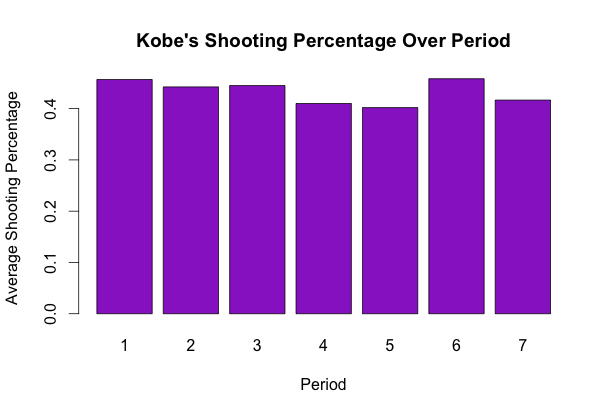
\includegraphics[width=14cm]{img/period}
\end{center}
Note that periods $5$ through $7$ refer to overtime periods. Kobe appears to be relatively consistent in his shooting percentage over the periods. There does not appear to be a marked improvement in his shooting in the latter periods. In fact, his lowest percentages are in the fourth, fifth and seventh periods, though his highest percentage is in the sixth period.  
\begin{center}
	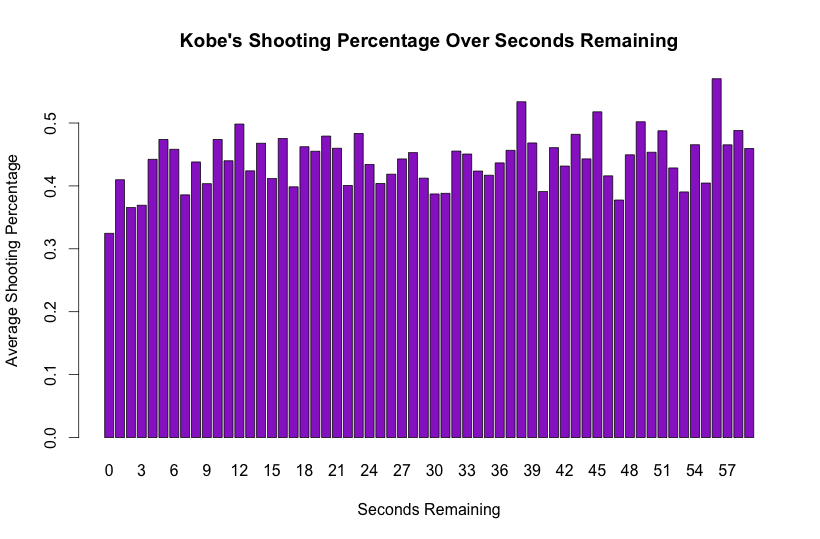
\includegraphics[width=14cm]{img/seconds}
\end{center}
Again Kobe appears to be relatively consistent in his shooting percentage in the last minute of play. However, his accuracy appears to dip dramatically when there are zero seconds left (shots made right at the buzzer).
\begin{center}
	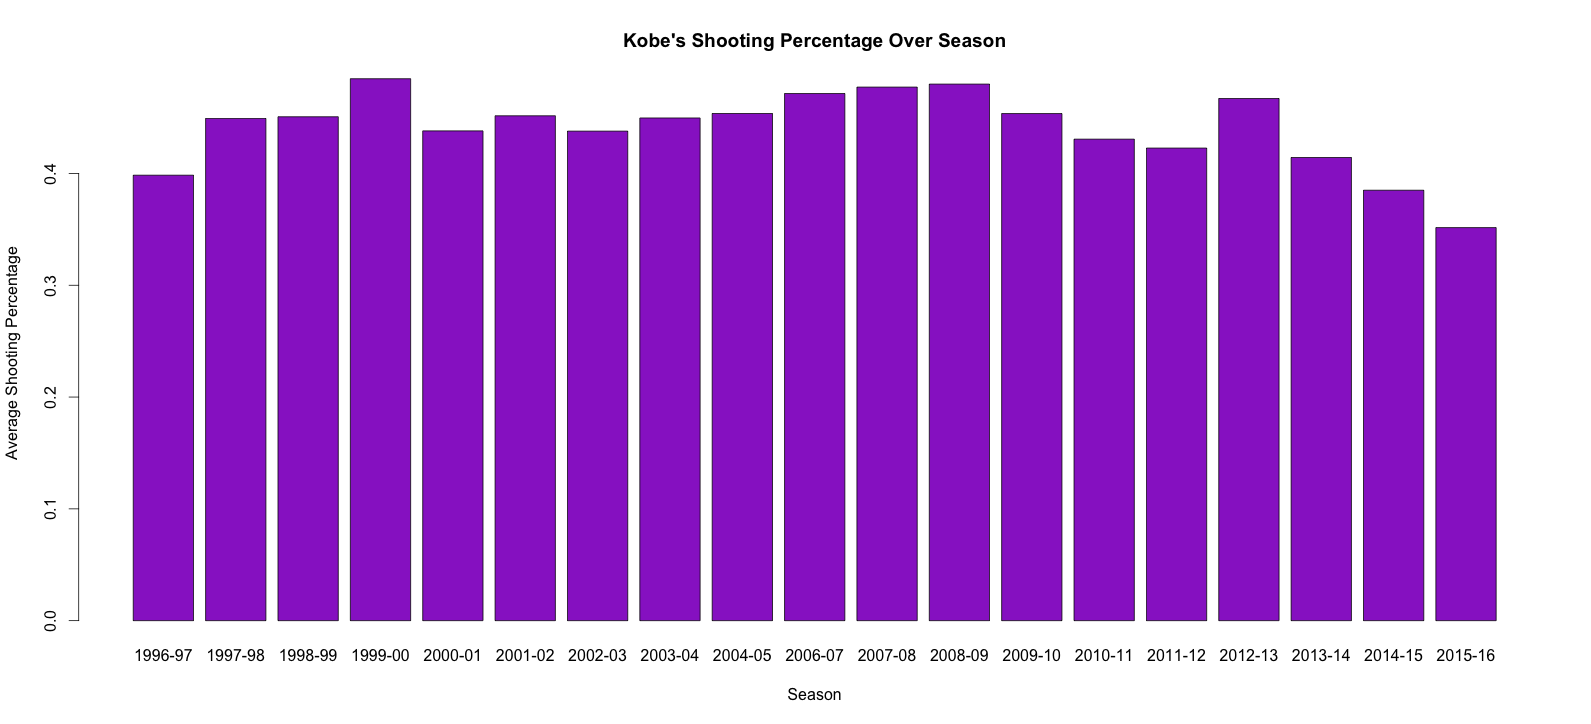
\includegraphics[width=19cm]{img/season}
\end{center}
Consistency again is the main trend when it comes to Kobe's shooting performance over season for most of his career. As expected, there is a noticeable decline in his final few seasons.
\begin{center}
	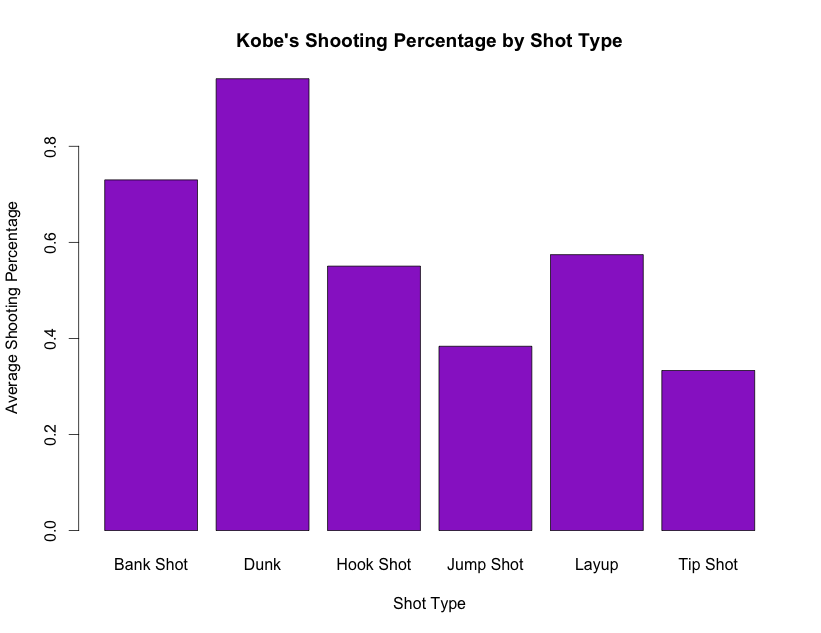
\includegraphics[width=14cm]{img/type}
\end{center}
Unsurprisingly, Kobe's most accurate shot is a dunk given the close range. His second most accurate shot is a bank shot and his least accurate shot is the jump shot, which makes sense given that this category would include three pointers.\\

After making these preliminary observations, we moved on to significance testing and model building.

\subsection{Significance Testing}
\subsection{Model Building}

\section{Limitations}
\subsection{Lack of Free-Throw Data}
\hspace*{1cm}One disadvantage of the dataset we utilized was that it only considered field goals during running game time i.e. 2-point and 3-point field goals. While free throws are often considered indicative of a player's effectiveness in clutch situations, in many ways regular field goals are more impressive because, unlike with free throws, players are challenged by their opponents when taking jump shots and layups. Thus, despite this specific absence in the dataset we feel that our analysis still reveals much about Kobe's overall effectiveness in normal and higher stress clutch conditions.
\section{Challenges Faced \& Lessons Learned}
\hspace*{1cm}One challenge we faced while performing data preprocessing was that the \texttt{date} variable obtained from scraping the win-loss data originally used a long-form format (e.g, ``May 2, 2016''). When we used Excel to change the date formatting and proceeded with the data cleaning in \texttt{cleaning.R}, we noticed that some of the dates were years in the future (which is clearly beyond the realm of possibility for basketball shots already taken by Kobe Bryant). To resolve this error, we passed in the raw data obtained by the scraping process into R, and discovered that R had a parsing option for long-form dates. Using the R-formatted dates, we were able to accurately merge the win-loss data with our shooting data. 

\hspace*{1cm}On the topic of data preprocessing, we learned that real-world data can be messy to work with. The data we had to work with from Kaggle was relatively clean to begin with, but even then we had to do some nontrivial preprocessing in order to suit our analysis.

\hspace*{1cm}In terms of performing analysis, one of our main takeaways was that given a large amount of data and features, it is a challenge to determine what sort of analysis to perform. There are many more potential statistical relationships we could have explored given the richness of the data set. That said, we believe that we have performed a reasonable amount of analysis for the goal of addressing our research questions.
\section{Conclusion}
\begin{thebibliography}{9}
	\bibitem{kagglecompetition}
	Kaggle. 
	\textit{Kobe Bryant Shot Selection}, \texttt{https://www.kaggle.com/c/kobe-bryant-shot-selection}

	\bibitem{forumpost}
	Kaggle. 
	\textit{Splitting of data into training and test},\\ \texttt{https://www.kaggle.com/c/DontGetKicked/forums/t/975/splitting-of-data-into-training-and-test}

	\bibitem{landofbasketball}
	Land of Basketball.com.
	\textit{Los Angeles Lakers}, \\\texttt{http://www.landofbasketball.com/teams/records\_los\_angeles\_lakers.htm}

\end{thebibliography}
\section*{Acknowledgements}
\hspace*{1cm}Special thanks to Phillip Huang for his kind assistance in helping us scrape win-loss data using the Web Scraper Chrome extension.

\end{document}